\documentclass[12pt,a4paper,notitlepage]{article}

\usepackage[utf8]{inputenc}

\usepackage[francais]{babel}\usepackage[T1]{fontenc}
\usepackage[cyr]{aeguill}
\usepackage{lmodern}
\usepackage{color}
\usepackage{boites}
\usepackage{fancybox}
\usepackage{listings}
\lstset{language=bash, basicstyle=\footnotesize, frame=shadowbox, rulesepcolor=\color{gris}}


\definecolor{gris}{gray}{0.75}
%\definecolor{bleup}{HTML}{258EE9}


%\renewcommand*\familydefault{\ttdefault} %% Only if the base font of the document is to be typewriter style
%\renewcommand{\rmdefault}{ptm}


\usepackage[
   pdfauthor={Ludovic Terrier & Arnaud Goulut},
   pdftitle={RE12 - TP2},
   ]{hyperref}
   
   
\usepackage[pdftex]{graphicx}

%\usepackage{titlesec}
%\titleformat{\section}[frame] {\normalfont} {\filright
%\footnotesize
%\enspace\textbf{\thesection}\enspace} {8pt} {\Large\bfseries\filcenter}

%% Je contrôle la taille de ma zone imprimée...
\usepackage{anysize}
%% ...en définissants les marges {gauche}{droite}{haute}{basse}
\marginsize{25mm}{15mm}{10mm}{15mm}

\begin{document}

\title{La résolution des noms}
\author{Arnaud Goulut et Ludovic Terrier}
\date{Avril 2010}
\maketitle


%\tableofcontents

\thispagestyle{empty}


%%%%%%%%%%%%%%%%%%%%%%%%%%%%%%%%%%%  1ère page 


%%%%%%%%%%%%%%%%%%%%%%%%%%%%%%%%%%% 1ère partie
\section{Partie 1 : Le DNS côté client}

\subsection{Le fichier \texttt{/etc/resolv.conf}}
Pour utiliser le DNS de l'UTT (ie. 193.50.230.240), il faut dans le fichier \texttt{/etc/resolv.conf} mettre : \\

\begin{lstlisting}
nameserver 193.50.230.240
search utt.fr
\end{lstlisting}

\bigskip
On peut utiliser deux directives dans ce fichier :
\begin{itemize}
\item search : ajoute automatiquement ce suffixe lors des résolutions
\item domain : définit le domaine auquel appartient la machine
\end{itemize}


\subsection{L'outils dig}
Dig peut être utiliser pour effectuer différents types de requêtes.

\subsubsection{Directe}

Une requête directe avec dig s'obtient avec la commande : \texttt{dig flickr.com in A}\\
\begin{lstlisting}
;; QUESTION SECTION:
;flickr.com.                    IN      A

;; ANSWER SECTION:
flickr.com.             335     IN      A       68.142.214.24

;; AUTHORITY SECTION:
flickr.com.             76681   IN      NS      ns2.yahoo.com.
flickr.com.             76681   IN      NS      ns5.yahoo.com.
flickr.com.             76681   IN      NS      ns3.yahoo.com.
flickr.com.             76681   IN      NS      ns1.yahoo.com.

;; Query time: 60 msec
;; SERVER: 212.27.40.241#53(212.27.40.241)
;; WHEN: Sat May  1 14:43:58 2010
;; MSG SIZE  rcvd: 140
\end{lstlisting}

\subsubsection{Inverse}
Une requête inverse avec dig s'obtient avec la commande : \texttt{dig -x 193.50.230.240}\\
\begin{lstlisting}
;; QUESTION SECTION:
;240.230.50.193.in-addr.arpa.   IN      PTR

;; ANSWER SECTION:
240.230.50.193.in-addr.arpa. 86400 IN   PTR     pluton.utt.fr.

;; AUTHORITY SECTION:
230.50.193.in-addr.arpa. 86400  IN      NS      pluton.utt.fr.
230.50.193.in-addr.arpa. 86400  IN      NS      orion.utc.fr.

;; Query time: 68 msec
;; SERVER: 212.27.40.241#53(212.27.40.241)
;; WHEN: Sat May  1 14:52:08 2010
;; MSG SIZE  rcvd: 110
\end{lstlisting}

\subsubsection{Mail exchange}
Une requête mail exchange avec dig s'obtient avec la commande : \texttt{dig }\\
\begin{lstlisting}
;; QUESTION SECTION:
;utbm.fr.                       IN      MX

;; ANSWER SECTION:
utbm.fr.                259200  IN      MX      1 serveur2314.utbm.fr.

;; AUTHORITY SECTION:
utbm.fr.                259200  IN      NS      pluton.utt.fr.
utbm.fr.                259200  IN      NS      portail1.utbm.fr.
utbm.fr.                259200  IN      NS      portail2.utbm.fr.
utbm.fr.                259200  IN      NS      portail5.utbm.fr.

;; ADDITIONAL SECTION:
serveur2314.utbm.fr.    259200  IN      A       193.48.231.4
portail1.utbm.fr.       600     IN      A       193.48.246.2
portail2.utbm.fr.       259200  IN      A       193.48.246.11
portail5.utbm.fr.       259200  IN      A       193.48.246.16

;; Query time: 84 msec
;; SERVER: 212.27.40.241#53(212.27.40.241)
;; WHEN: Sat May  1 15:03:15 2010
;; MSG SIZE  rcvd: 211
\end{lstlisting}


\clearpage
\subsection{L'outil whois}
Cette commande permet de modifier le paramétrage des différents services dont celui du réseau. On peut tout d'abord vérifier les états au démarrage d'un service donné pour chaques runlevels avec la commande :\\

\begin{lstlisting}
Domain ID:D101496757-LROR
Domain Name:FEDORAPROJECT.ORG
Created On:24-Sep-2003 10:32:11 UTC
Last Updated On:23-Jul-2009 17:52:39 UTC
Expiration Date:24-Sep-2010 10:32:11 UTC
Sponsoring Registrar:Network Solutions LLC (R63-LROR)
Status:CLIENT TRANSFER PROHIBITED
Registrant ID:41295926-NSI
Registrant Name:Red Hat, Inc.
Registrant Organization:Red Hat, Inc.
Registrant Street1:1801 Varsity Drive
Registrant City:Raleigh
Registrant State/Province:NC
Registrant Postal Code:27606
Registrant Country:US
Registrant Phone:+1.919754370
Registrant FAX:+1.919754370
Registrant Email:domainadmin@redhat.com
Admin ID:41295926-NSI
Admin Name:Red Hat, Inc.
Admin Organization:Red Hat, Inc.
Admin Street1:1801 Varsity Drive
Admin City:Raleigh
Admin State/Province:NC
Admin Postal Code:27606
Admin Country:US
Admin Phone:+1.919754370
Admin FAX:+1.919754370
Admin Email:domainadmin@redhat.com
Tech ID:41434783-NSI
Tech Name:Fedora Project
Tech Street1:Red Hat
Tech Street2:1801 Varsity Drive
Tech City:Raleigh
Tech State/Province:NC
Tech Postal Code:27606
Tech Country:US
Tech Phone:+1.919754370
Tech Email:admin@fedora.redhat.com
Name Server:NS1.FEDORAPROJECT.ORG
Name Server:NS2.FEDORAPROJECT.ORG
DNSSEC:Unsigned
\end{lstlisting}

\clearpage
\section{Partie 2 : Mise en \oe uvre d'un serveur relai}
Le serveur
\subsection{Installation de Bind9}

\begin{lstlisting}
options {
        listen-on port 53 { 192.168.3.129; };
        listen-on-v6 port 53 { ::1; };
        directory       "/var/named";
        dump-file       "/var/named/data/cache_dump.db";
        statistics-file "/var/named/data/named_stats.txt";
        memstatistics-file "/var/named/data/named_mem_stats.txt";
        allow-query     { localhost; 192.168.3.0/24; };
        recursion yes;
        forward first;
        forwarders {
        193.50.230.240 port 53;
        };
};

logging {
        channel default_debug {
                file "data/named.run";
                severity dynamic;
        };
};

zone "." IN {
        type hint;
        file "named.ca";
};

include "/etc/named.rfc1912.zones";
\end{lstlisting}

\subsection{Configuration du resolver}
Il suffit de remplacer l'adresse IP de l'ancien DNS présent dans le fichier \texttt{/etc/resolv.conf} par celle du serveur faisant office de relai. 

\subsection{Fonctionnement du relai}

\begin{figure}[!h]
\begin{center}
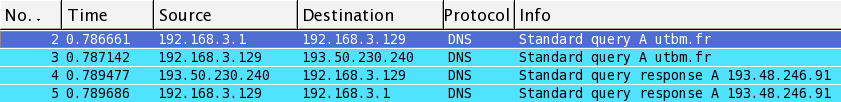
\includegraphics[scale=0.61]{capture-via-relai}
\caption{Requête DNS via un relai.}
\label{fig:da}
\end{center}
\end{figure}



\section{Partie 3 : Résolution du domaine b3.re12.fr}

\subsection{Configuration}

Pour pouvoir gérer la zone b3.re12.fr il faut effectuer deux opérations :
\begin{itemize}
\item ajouter dans le fichier \texttt{/etc/named.conf} la gestion de cette zone
\item créer le fichier contenant l'ensemble des paramètres de la zone
\end{itemize}

\bigskip

\subsubsection{Modification du fichier \texttt{/etc/named.conf}}

\begin{lstlisting}
zone "b3.re12.fr" IN {
        type master;
        file "db.b3.re12.fr";
};
\end{lstlisting}

\subsubsection{Création du fichier \texttt{/var/named/b3.re12.fr}}

\begin{lstlisting}
$TTL 3h
@       IN      SOA     ns.b3.re12.fr. hostmaster.b3.re12.fr. (
                                2005090202
                                8H
                                2H
                                1W
                                1D )

@       IN      NS      ns.b3.re12.fr.

@       IN      MX   10   mail.b3.re12.fr.

pc-arnaud       IN A 192.168.3.1
pc-ludo         IN A 192.168.3.129
router-ludo     IN A 192.168.3.254
router-arnaud   IN A 192.168.3.126
ns              IN NS 192.168.3.129
mail            IN A 192.168.3.129
\end{lstlisting}

\clearpage
\subsection{La résolution inverse}

\subsubsection{Modification du fichier \texttt{/etc/named.conf}}

\begin{lstlisting}
zone "3.168.192.in-addr.arpa" IN {
        type master;
        file "db.3.168.192.in-addr.arpa";
};
\end{lstlisting}

\subsubsection{Création du fichier \texttt{/var/named/db3.inv}}

\begin{lstlisting}
$TTL    604800
@       IN      SOA     ns.b3.re12.fr. root.b3.re12.fr.     (
                2010042701 ; Serial (date + incrementation)
                7200       ; Refresh
                3600       ; Retry
                1209600    ; Expire
                604800     ; Negative Cache TTL
                )

A 192.168.3.1
A 192.168.3.129
A 192.168.3.254
A 192.168.3.126
NS 192.168.3.129
A 192.168.3.129

1                 PTR     pc-arnaud
129               PTR     pc-ludo
254               PTR     router-ludo
126               PTR     router-arnaud
\end{lstlisting}


\end{document}